<<<<<<< HEAD
\documentclass[
  bibliography=totoc,     % Literatur im Inhaltsverzeichnis
  captions=tableheading,  % Tabellenüberschriften
  titlepage=firstiscover, % Titelseite ist Deckblatt
]{scrartcl}

% Paket float verbessern
\usepackage{scrhack}

% Warnung, falls nochmal kompiliert werden muss
\usepackage[aux]{rerunfilecheck}

% unverzichtbare Mathe-Befehle
\usepackage{amsmath}
% viele Mathe-Symbole
\usepackage{amssymb}
% Erweiterungen für amsmath
\usepackage{mathtools}
%einheiten einfügen

% Fonteinstellungen
\usepackage{fontspec}
% Latin Modern Fonts werden automatisch geladen
% Alternativ zum Beispiel:
%\setromanfont{Libertinus Serif}
%\setsansfont{Libertinus Sans}
%\setmonofont{Libertinus Mono}

% Wenn man andere Schriftarten gesetzt hat,
% sollte man das Seiten-Layout neu berechnen lassen
\recalctypearea{}

% deutsche Spracheinstellungen
\usepackage[main=ngerman]{babel}


\usepackage[
  math-style=ISO,    % ┐
  bold-style=ISO,    % │
  sans-style=italic, % │ ISO-Standard folgen
  nabla=upright,     % │
  partial=upright,   % ┘
  warnings-off={           % ┐
    mathtools-colon,       % │ unnötige Warnungen ausschalten
    mathtools-overbracket, % │
  },                       % ┘
]{unicode-math}

% traditionelle Fonts für Mathematik
\setmathfont{Latin Modern Math}
% Alternativ zum Beispiel:
%\setmathfont{Libertinus Math}

\setmathfont{XITS Math}[range={scr, bfscr}]
\setmathfont{XITS Math}[range={cal, bfcal}, StylisticSet=1]

% Zahlen und Einheiten
\usepackage[
  locale=DE,                   % deutsche Einstellungen
  separate-uncertainty=true,   % immer Fehler mit \pm
  per-mode=symbol-or-fraction, % / in inline math, fraction in display math
]{siunitx}

% chemische Formeln
\usepackage[
  version=4,
  math-greek=default, % ┐ mit unicode-math zusammenarbeiten
  text-greek=default, % ┘
]{mhchem}

% richtige Anführungszeichen
\usepackage[autostyle]{csquotes}

% schöne Brüche im Text
\usepackage{xfrac}

% Standardplatzierung für Floats einstellen
\usepackage{float}
\floatplacement{figure}{htbp}
\floatplacement{table}{htbp}

% Floats innerhalb einer Section halten
\usepackage[
  section, % Floats innerhalb der Section halten
  below,   % unterhalb der Section aber auf der selben Seite ist ok
]{placeins}

% Seite drehen für breite Tabellen: landscape Umgebung
\usepackage{pdflscape}

% Captions schöner machen.
\usepackage[
  labelfont=bf,        % Tabelle x: Abbildung y: ist jetzt fett
  font=small,          % Schrift etwas kleiner als Dokument
  width=0.9\textwidth, % maximale Breite einer Caption schmaler
]{caption}
% subfigure, subtable, subref
\usepackage{subcaption}


% Grafiken können eingebunden werden
\usepackage{graphicx}
% größere Variation von Dateinamen möglich
%\usepackage{grffile}

% schöne Tabellen
\usepackage{booktabs}

% Verbesserungen am Schriftbild
\usepackage{microtype}
\setlength{\parindent}{0pt}

% Literaturverzeichnis
\usepackage[
  backend=biber,
]{biblatex}
% Quellendatenbank
\addbibresource{lit.bib}
\addbibresource{programme.bib}

% Hyperlinks im Dokument
\usepackage[
  german,
  unicode,        % Unicode in PDF-Attributen erlauben
  pdfusetitle,    % Titel, Autoren und Datum als PDF-Attribute
  pdfcreator={},  % ┐ PDF-Attribute säubern
  pdfproducer={}, % ┘
]{hyperref}
% erweiterte Bookmarks im PDF
\usepackage{bookmark}

% Trennung von Wörtern mit Strichen
\usepackage[shortcuts]{extdash}

% Import PDFs
\usepackage{pdfpages}


\author{%
  Konstantin Mrozik\\%
  \href{mailto:konstantin.mrozik@udo.edu}{konstantin.mrozik@udo.edu}%
  \and%
  Marcel Kebekus\\%
  \href{mailto:marcel.kebekus@udo.edu}{marcel.kebekus@udo.edu}%
}
\publishers{TU Dortmund – Fakultät Physik}


\title{Zusatzversuch bei Firma Schnöring}
\author{%
  Konstantin Mrozik\\%
  \href{mailto:konstantin.mrozik@tu-dortmund.de}{konstantin.mrozik@tu-dortmund.de}%
  \and%
  Marcel Kebekus\\%
  \href{mailto:marcel.kebekus@tu-dortmund.de}{marcel.kebekus@tu-dortmund.de}%
}
\date{%
  Durchführung: 18.02.2020
  \hspace{3em}
  Abgabe: 
}
\publishers{TU Dortmund – Fakultät Physik}
\makeatletter         
\def\@maketitle{
\raggedright
\includegraphics[width=\textwidth]{bilder/lo_TU-Do 2008/logo_rgb_jpg}\\[8ex]
\begin{center}
{\Huge \bfseries \sffamily \@title }\\[4ex] 
{\Large  \@author}\\[4ex] 
\@date\\[8ex]
\publishers\\
\end{center}}
\makeatother


\begin{document}


\maketitle
\thispagestyle{empty}
\tableofcontents
\newpage
\section{Theorie}
\label{sec:Theorie}
Die Fourier Synthese ist eine Methode um eine beliebige Funktion mit einer Summe von Kosinus und Sinus Funktionen zu approximieren.
\begin{align}
    f(t) &= \sum_{k=0}^{\infty} (A_k\cos(\omega_k t)+B_k\sin(\omega_k t)) &   mit \; \omega_k &= \frac{2\pi k}{T}
\end{align}
wobei die Koeffizienten $A_k$ und $B_k$ festgelegt sind durch
\begin{align}
    A_k &= \frac{2}{T} \int_{-T/2}^{+T/2} f(t)\cos(\omega_k t) dt    &  mit \; A_0 &= \frac{1}{T} \int_{-T/2}^{+T/2} f(t) dt \\
    B_k &= \frac{2}{T} \int_{-T/2}^{+T/2} f(t)\sin(\omega_k t) dt    &  mit \; B_0 &= 0
\end{align}
\\
Dabei beschreibt $T$ die Periodendauer, $\omega_k$ die Frequenz und $A_k$ und $B_k$ die zugehörigen Koeffizienten. \\
Im Folgenden soll mit dem Programm Fouriersynthese %Bib setzen
die Funktionen $f(x)=x$ und $f(x)=|sin(x)|$ nachgestellt und die jeweilligen Koeffizienten $B_k$ und $A_k$ ermittelt werden.

\newpage
\section{Durchführung}
\label{sec:Durchfuehrung} %darauf wird verlinkt in Vorbereitungsteil Elastisches Nachwirken!
\subsection{Versuchsaufbau}

\begin{figure}[h]
    \begin{subfigure}[c]{0.5\textwidth}
        \centering
        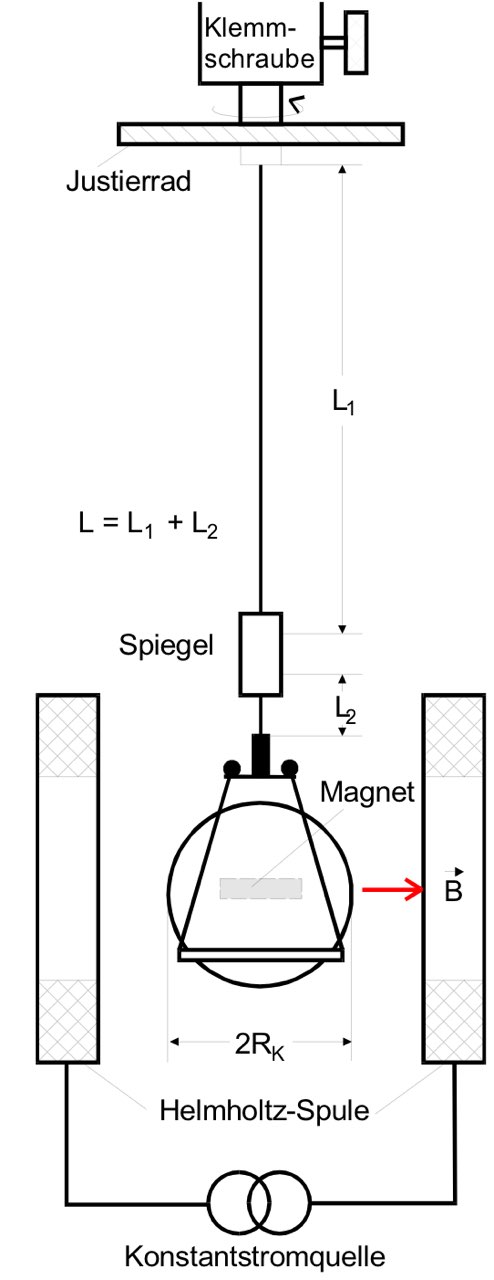
\includegraphics[width=0.3\textwidth, height=0.7\textwidth]{bilder/magnet_apperatur.jpeg}
        \subcaption{Versuchsaufbau Skizze,\cite[9]{Anleitung}}        
        \label{fig:Torsion_apperatur}
    \end{subfigure}
    \begin{subfigure}[c]{0.5\textwidth}
        \centering
        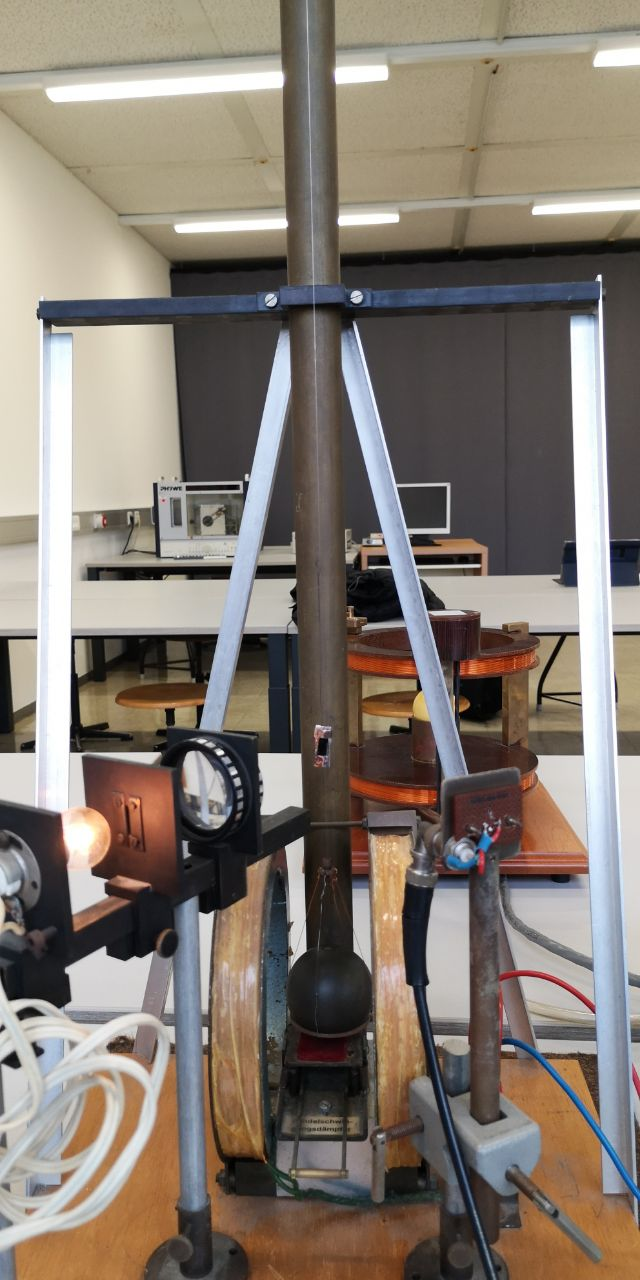
\includegraphics[width=0.3\textwidth, height=0.7\textwidth]{bilder/Foto_Versuchsaufbau.jpeg}
        \subcaption{Foto des Versuchsaufbaus}
        \label{fig:Foto_Versuchsaufbau}
    \end{subfigure}
\end{figure}

Die Kugel soll im Versuch nicht pendeln um Fehler in den Versuchswerten zu vermeiden.
Daher ist unter der Kugel eine Vorrichtung angebracht um nach jeder Messreihe die Pendelbewegung zu dämpfen.\\

Um die Periodendauer zu messen muss mithilfe des Rings an der Aufhängung des Drahtes der Draht verdreht werden,
wobei darauf geachtet werden muss dass der Spiegel bei der Schwingung den Lichtstrahl über die Photodiode lenkt.\\

Das Experiment zur Bestimmung des Elastizitätsmoduls aus der Schallgeschwindigkeit war nicht durchführbar,
daher haben wir hierfür einen vorgegebenen Wert erhalten.\\

\subsection{Die Periodendauer T}
Im ersten Versuch darf an der Helmholtzspule kein Strom anliegen da ausschließlich die Elastizität des Stoffes
 Einfluss auf die Periodendauer haben soll.
Zu Beginn des Versuches wird der Magnet im inneren der Kugel parallel zum Draht eingestellt.
Die Lampe am Versuchsaufbau wird eingeschaltet und das Licht trifft über eine Linse auf den am Draht befestigten Spiegel.
Wenn der Draht nun ausgelenkt wird, läuft der Lichtstrahl über den mitschwingenden Spiegel periodisch über die Photodiode.\\
Die Photodiode ist über eine elektrische Schaltung an die Quarzuhr gekoppelt.
Die elektrische Schaltung lässt über eine bistabile Kippstufe (Flip-Flop) das erste Signal passieren um die Stoppuhr zu starten.
Mithilfe einer weiteren bistabilen Kippstufe wird das 2. Signal unterdrückt.
Das dritte Signal stoppt die Quarzuhr und durch die monostabile Kippstufe und einen weiteren Flip-Flop wird die Uhr mit dem 4. Signal zurück gesetzt.\\
\begin{figure}[h]
    \begin{subfigure}[c]{0.5\textwidth}
        \centering
        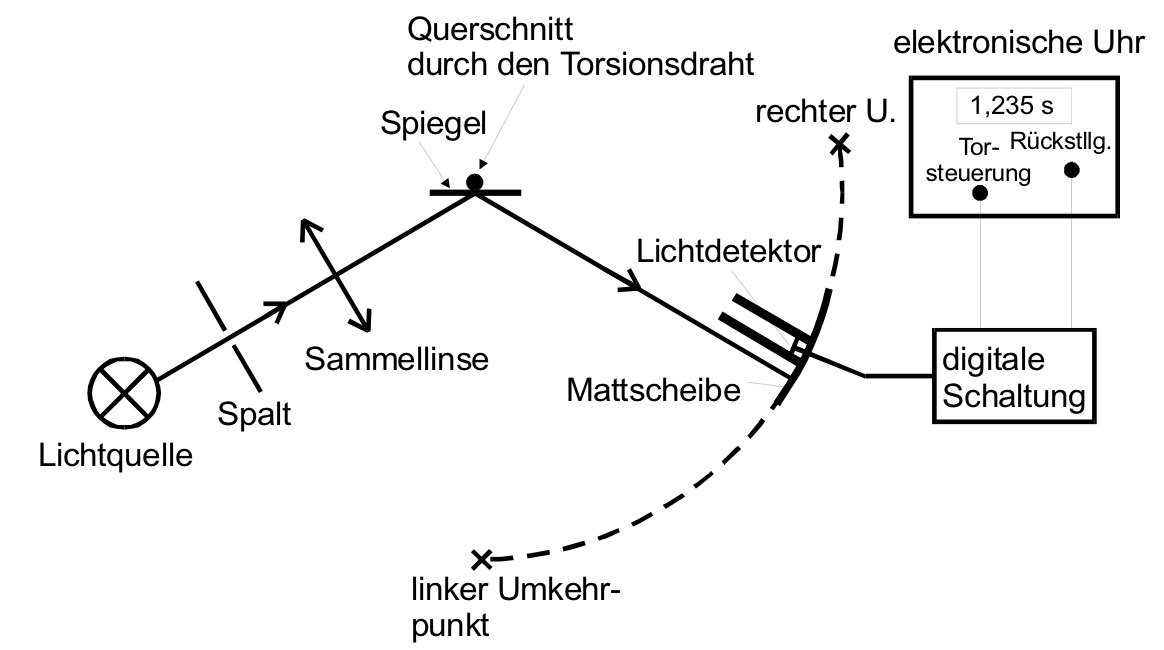
\includegraphics[width=0.7\textwidth, height=0.6\textwidth]{bilder/lichtuhr.jpeg}
        \subcaption{Lichtuhr Skizze,\cite[9]{Anleitung}}        
        \label{fig:lichtuhr}
    \end{subfigure}
    \begin{subfigure}[c]{0.5\textwidth}
        \centering
        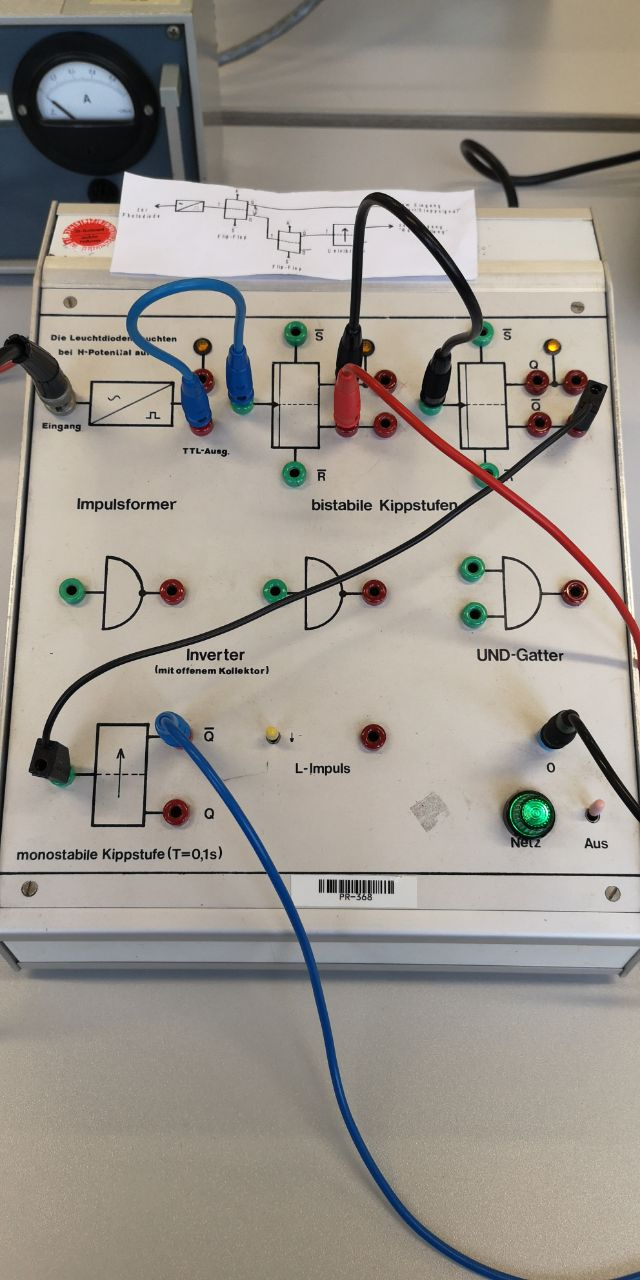
\includegraphics[width=0.45\textwidth, height=0.6\textwidth]{bilder/Schaltung.jpeg}
        \subcaption{Foto der Schaltung}
        \label{fig:Schaltung}
    \end{subfigure}
\end{figure}


\subsection{Die Periodendauer T im B-Feld}
Um die Stärke des Permanentmagneten in der Kugel zu berechnen muss dieser senkrecht zum Draht ausgerichtet werden, da so die Fehler durch das Erdmagnetfeld minimiert werden.
Die Stromstärke an der Helmholtzspule wird nun von 0.1 Ampere bis 1 Ampere in 0.1 Ampere Schritten erhöht und für jede Stromstärke werden 10 Werte gemessen.
\section{Auswertung}
\label{sec:Auswertung}
\subsection{Bestimmung der Brennweite aus Gegenstandsweite und Bildweite}
Aus dem Mittelwert der gemessenen Werte wird mithilfe von Gleichung \ref{eqn:linsengl} die Brennweite der Linse bestimmt.
\begin{equation}
    f_1 = \frac{g \cdot b}{g+b} = 95,86 \text{mm} \nonumber
\end{equation}
Die Messung wird nun über das auftragen der Messwerte in einem Koordinatensystem bewertet, wenn die Messgenauigkeit hoch ist, sollten sich alle geraden in einem Punkt schneiden dessen x und y koordinate der Brennwite entsprechen.
\begin{figure}[H]
    \centering
    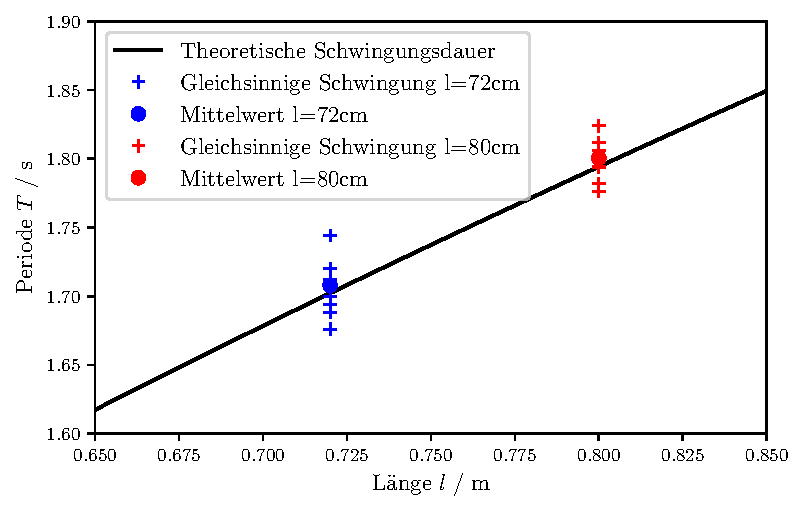
\includegraphics[width=0.6\textwidth]{plots/plot1.pdf}
    \caption{Die Wertepaare werden auf der jeweiligen Achse aufgetragen und durch eine Gerade verbunden}
\end{figure}
Die selbe Methode wird nun auf eine andere Linse mit einer anderen Brennweite angewandt.
Es ergibt sich:
\begin{equation}
    f_2 = 48,07 \text{mm} \nonumber
\end{equation}
Und der entsprachende Graph:
\begin{figure}[H]
    \centering
    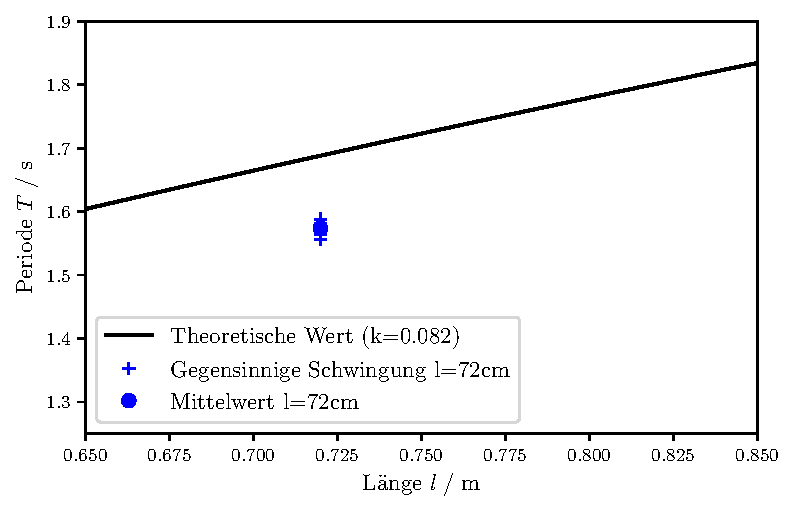
\includegraphics[width=0.6\textwidth]{plots/plot2.pdf}
    \caption{Die Wertepaare werden auf der jeweiligen Achse aufgetragen und durch eine Gerade verbunden}
\end{figure}

\subsection{Methode von Bessel}
Nach der Methode von Bessel lässt sich mit Gleichung \ref{eqn:bessel} die Brennweite der Linse bestimmen.
\begin{table}[H]
    \centering
    \begin{tabular}{c c | c }
        \toprule
        e & d & f\\
        mm & mm & mm\\
        \midrule
        400 & 70 & 96,94\\
        410 & 95 & 97,00\\
        420 & 119& 96,57\\
        430 & 138& 96,43\\
        440 & 155& 96,35\\
        450 & 170& 96,44\\
        460 & 182& 97,00\\
        470 & 193& 97,69\\
        480 & 211& 96,81\\
        490 & 221& 97,58\\
        500 & 233& 97,86 \\
        \bottomrule
    \end{tabular}
    \caption{Die Parameter e und b und die jeweilige berechnete Brennweite}
    \label{tab:tab1}
\end{table}
Als Mittelwert der berechneten Brennweiten ergibt sich
\begin{equation}
    f_{\text{bessel}} = 96,97 \text{mm} \nonumber
\end{equation}
\subsection{Methode von Abbe}
Bei der Methode von Abbe werden die g' und b' aus Gleichung \ref{eqn:abbe1} und \ref{eqn:abbe2} gegen den ensprechenden Term mit V aufgetragen und der lineare Zusammenhang wird untersucht.
\begin{figure}[H]
    \centering
    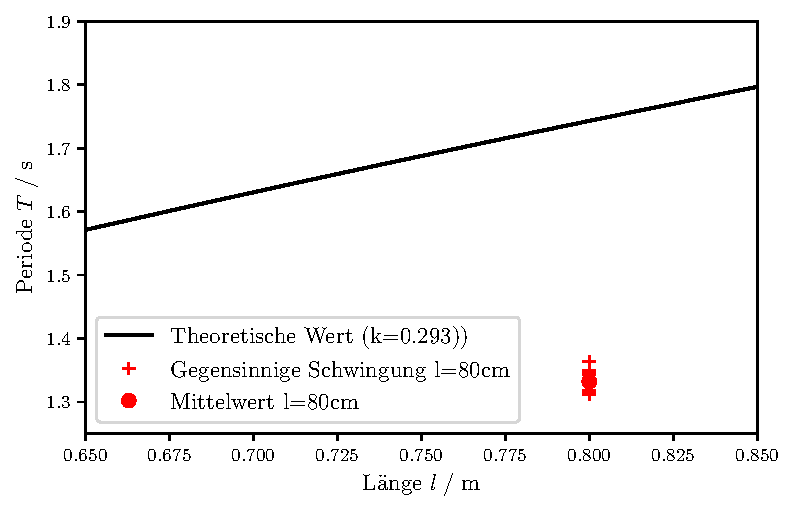
\includegraphics[width=0.6\textwidth]{plots/plot3.pdf}
    \caption{Abbe}
\end{figure}
\begin{figure}[H]
    \centering
    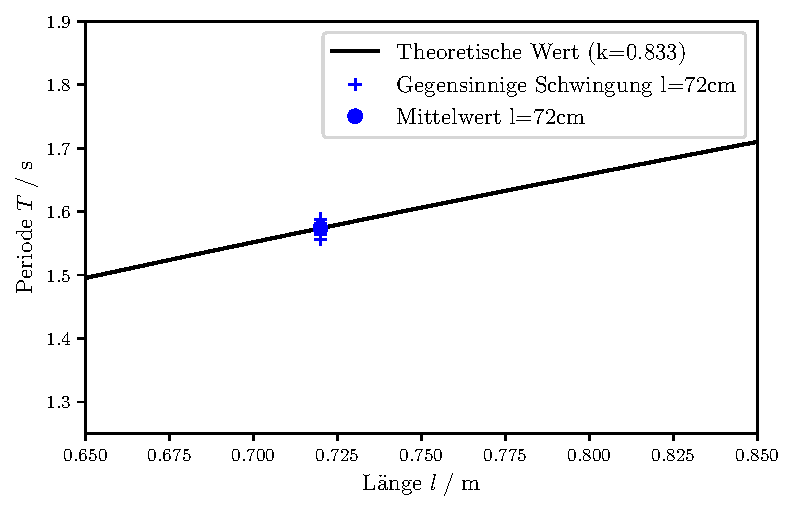
\includegraphics[width=0.6\textwidth]{plots/plot4.pdf}
    \caption{Abbe}
\end{figure}
Bei den hier gemessenen Werten lässt sich nur schwer ein linearer Zusammenhang erkennen.
\section{Diskussion}
\label{sec:Diskussion}

In der Auswertung kam es bereits zu einigen unrealistischen und offensichtlichen
falschen Werten die alle aus Berechnungen stammten.
Im Folgenden soll die Ursache für die dramastischen Abweichungen analysiert werden.


Dafür soll zu Beginn die Messung an sich überprüft werden.
Dazu wird die jeweilige theoretische Schwingungsdauer mit den gemessenen Schwingungsdauern verglichen.
\begin{figure}
    \centering
    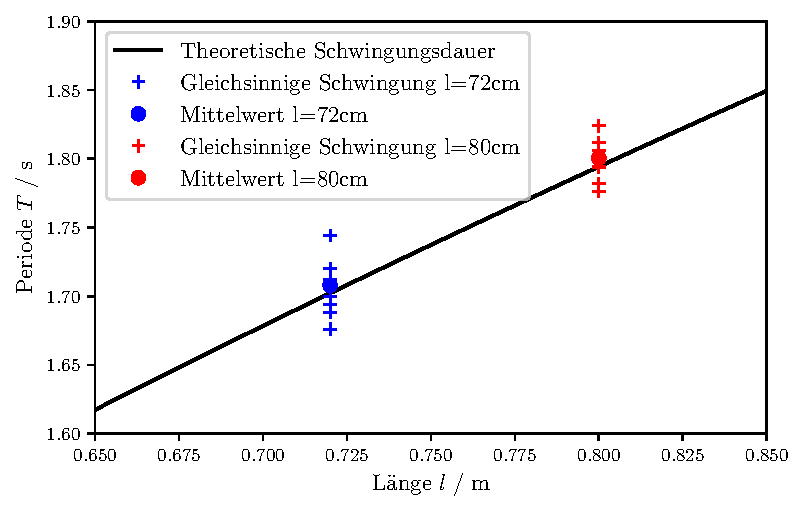
\includegraphics[width=0.5\textwidth]{plots/plot1.pdf}
    \caption{Gleichsinnige Schwingungen}
\end{figure}
Die Theoretische Kurve folgt aus Glichung (6!). Es wird deutlich, dass die gemessenen
Schwingungsdauern $T_+$ mit den zu erwartenen Schwingungsdauern übereinstimmt.\\

Für die Gegensinnige Schwingung ergibt sich der zu erwartende Theoretische Werte aus Geichung (8!).

\begin{figure}
    \begin{subfigure}[c]{0.5\textwidth}
        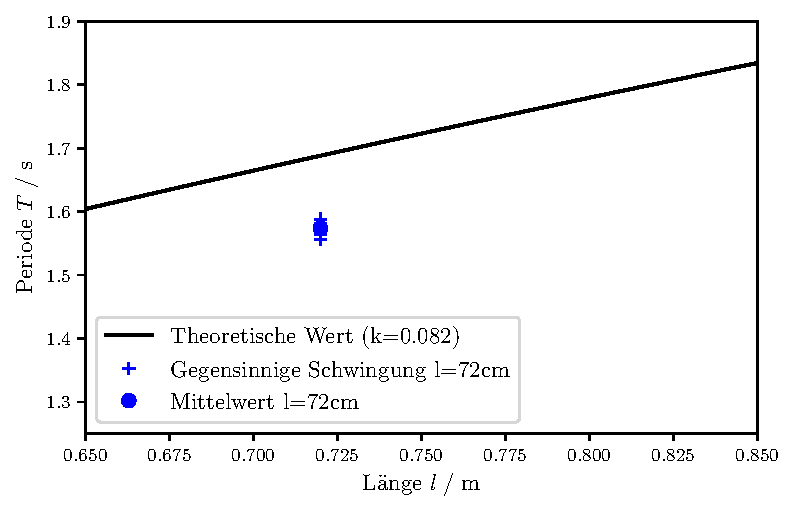
\includegraphics[width=\textwidth]{plots/plot2.pdf}
        \subcaption{Pedel 72cm}
    \end{subfigure}
    \begin{subfigure}[c]{0.5\textwidth}
        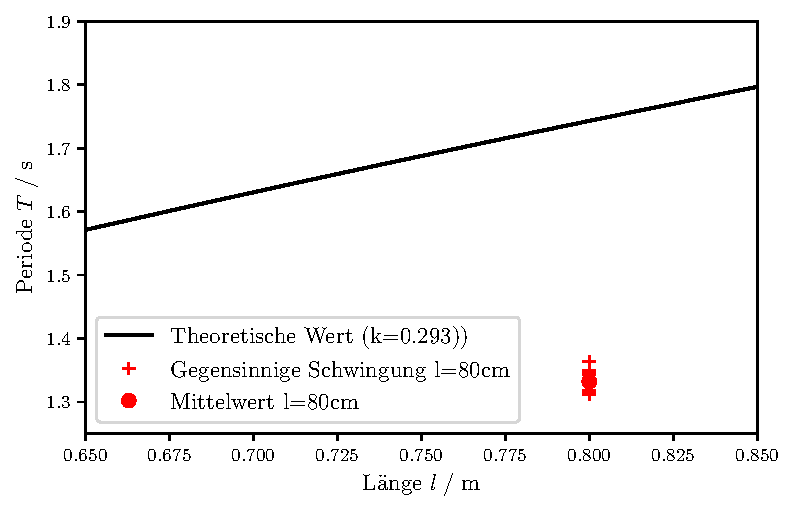
\includegraphics[width=\textwidth]{plots/plot3.pdf}
        \subcaption{Pendel 80cm}
        \label{subfig:pedel80}
    \end{subfigure}
    \caption{Gegensinnige Schwingungsdauer}
\end{figure}

Hier bei wird besonders gut deutlich, dass bei \ref{subfig:pendel80}, große Abweichungen
vorliegen. Dies lässt sich nur auf einen Messfehler zurückführen.
Weiterführend sei zu beachten, dass die Kopplungskonstante die für die theoretische Kurve
verwendet wird, ebenfalls aus diesen falschen Werten stammt.

Dies erklärt weiterführend, warum die Kopplungskonstant aus \ref{eqn:kopplung80} nicht die selben
sind.
Behauptung: Der Messfehler der Gegensinnigen Schwingung von der Pendellänge $l=80cm$ und $l=72cm$ ist 
ist ein Ursprung der Fehler.

Stellt man Gleichung (\ref{eqn:T_m}) um, um die Größenordung der Kopplungskonstante $K$ zu erörtern, so gilt:
\begin{equation}
    K=\frac{2\pi^2l}{T_{-}^2}-\frac{g}{2}
\end{equation}
Somit ergibt sich:
\begin{align*}
    \textrm{K für 72cm} = 0,833\\
    \textrm{K für 80cm} = 3,995 
\end{align*}
Für diese neuen Kopplungskonstanten sei gesagt, dass sie nur als Größenordnung diehnen.
Denn durch die passenden gleichsinnigen Schwingungsdauern $T_+$und den fehlerhaften gegensinnigen Schwingungsdauern $T_-$
folgt nach Gleichung (\ref{eqn:Kopplungkonstante}) eine fehlerhaft Kopplungkonstante $K$.
 
Trägt man für diese neuen Kopplungskonstanten die gegensinnigen Schwingungen auf, dies Bestätig die Annahme
das der Fehler in den gemessenen gegenphasigen Schwingungsdauern.  
\begin{figure}
    \begin{subfigure}[c]{0.5\textwidth}
        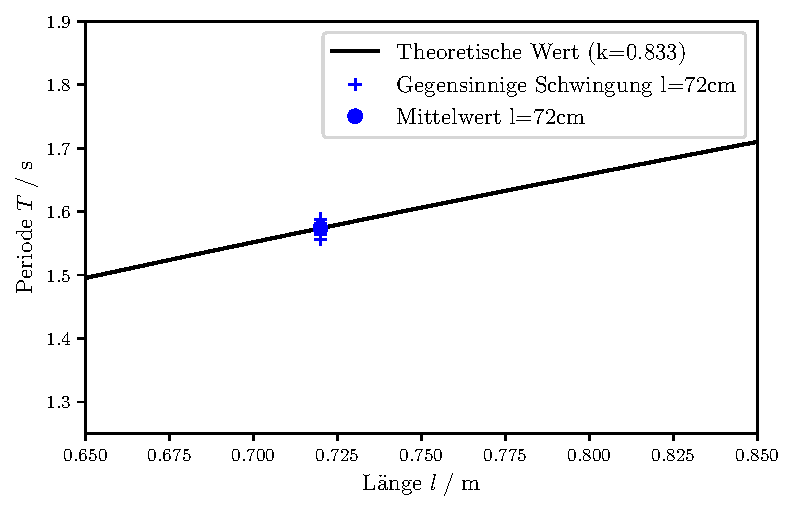
\includegraphics[width=\textwidth]{plots/plot4.pdf}
        \subcaption{Pedel 72cm}
    \end{subfigure}
    \begin{subfigure}[c]{0.5\textwidth}
        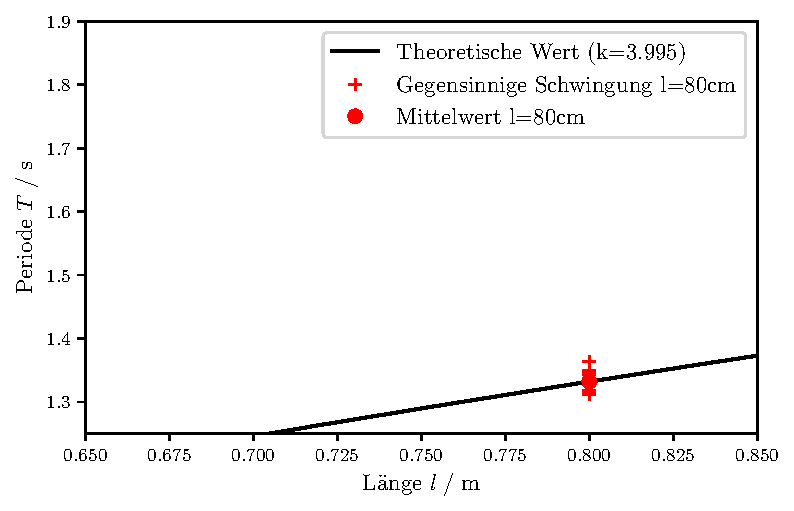
\includegraphics[width=\textwidth]{plots/plot5.pdf}
        \subcaption{Pendel 80cm}
        \label{subfig:gegenNEU80}
    \end{subfigure}
    \caption{Gegensinnige Schwingungsdauer mit Kopplungskonstante}
\end{figure}

Fazit: Der Fehler findet sich beim Messen der gegensinnigen Schwingungen und
zieht sich dann durch die Rechnungen für die Kopplungskonstante $K$ und die Frequenzen $\omega$
so wie für die Schwebungsdauer.\\
Somit stimmen gemessene und berechnete Werte nicht überein.



\section{Anhang}
\label{sec:anhang}
\subsection{Federberechnung der Firma Schnöring}
\begin{center}
    \makebox[\textwidth]{
        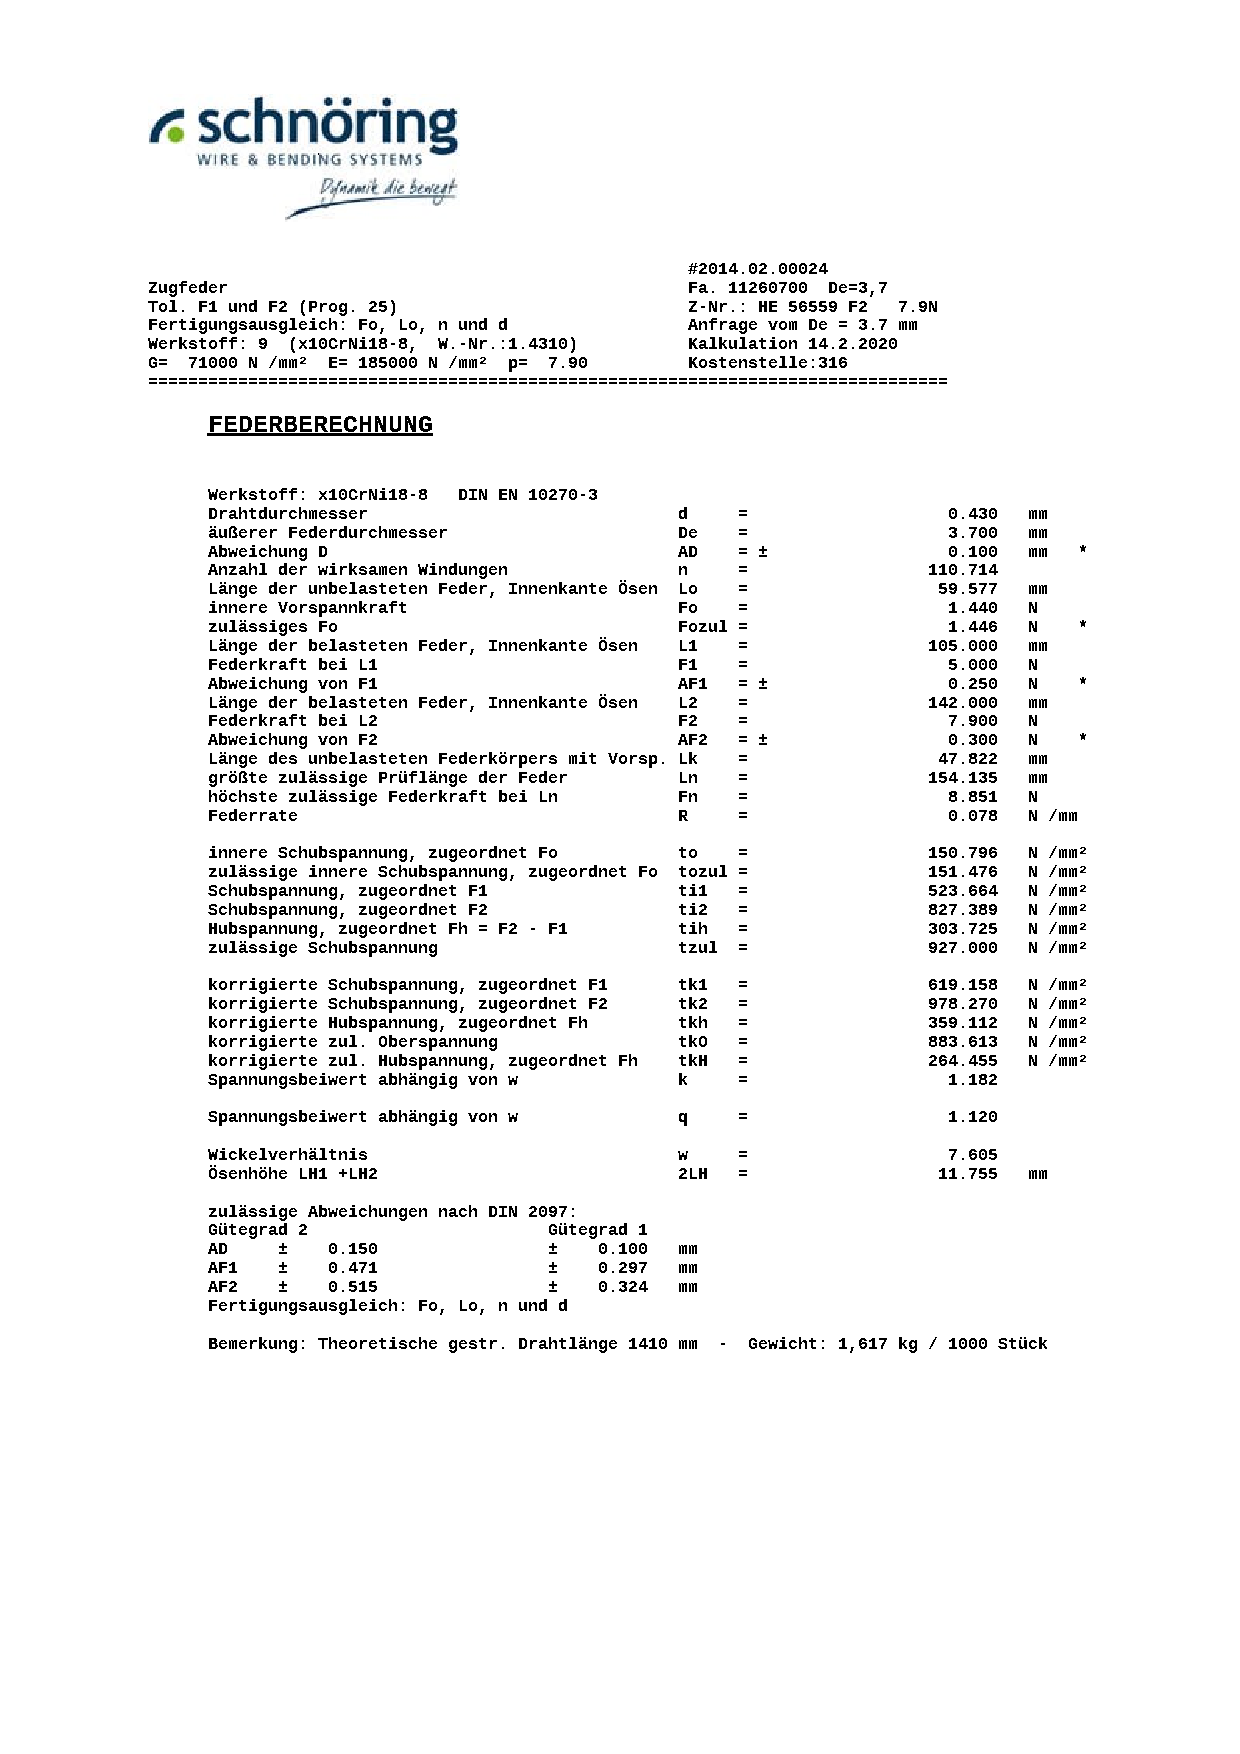
\includegraphics[width=\paperwidth]{bilder/berechnung_De_37.pdf}
        \label{fig:schn_b37}
        }
\end{center}
%\subsection{Eigene Federberechnung\cite{Programm}}
%\begin{center}
%    \makebox[\textwidth]{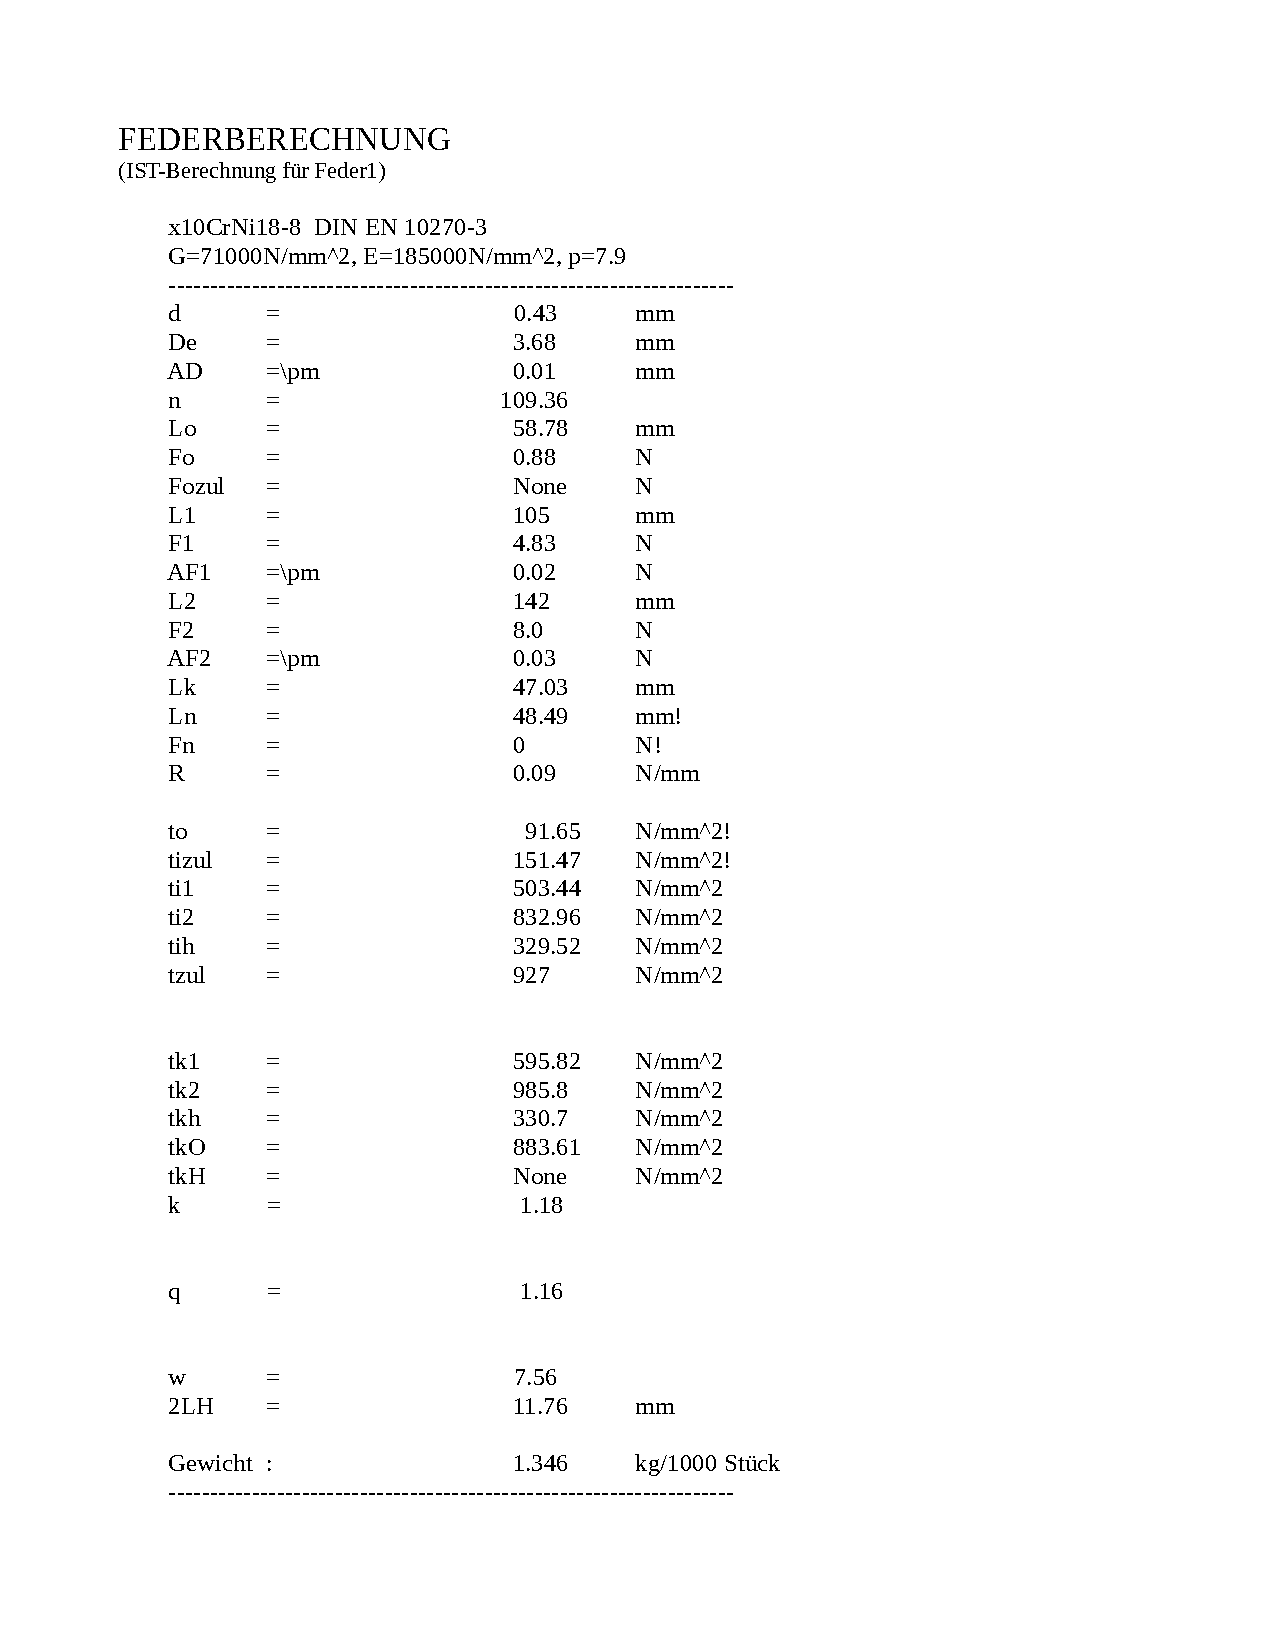
\includegraphics[width=\paperwidth]{bilder/my_berechnung368.pdf}}
%\end{center}


%\begin{center}
%    \makebox[\textwidth]{
%        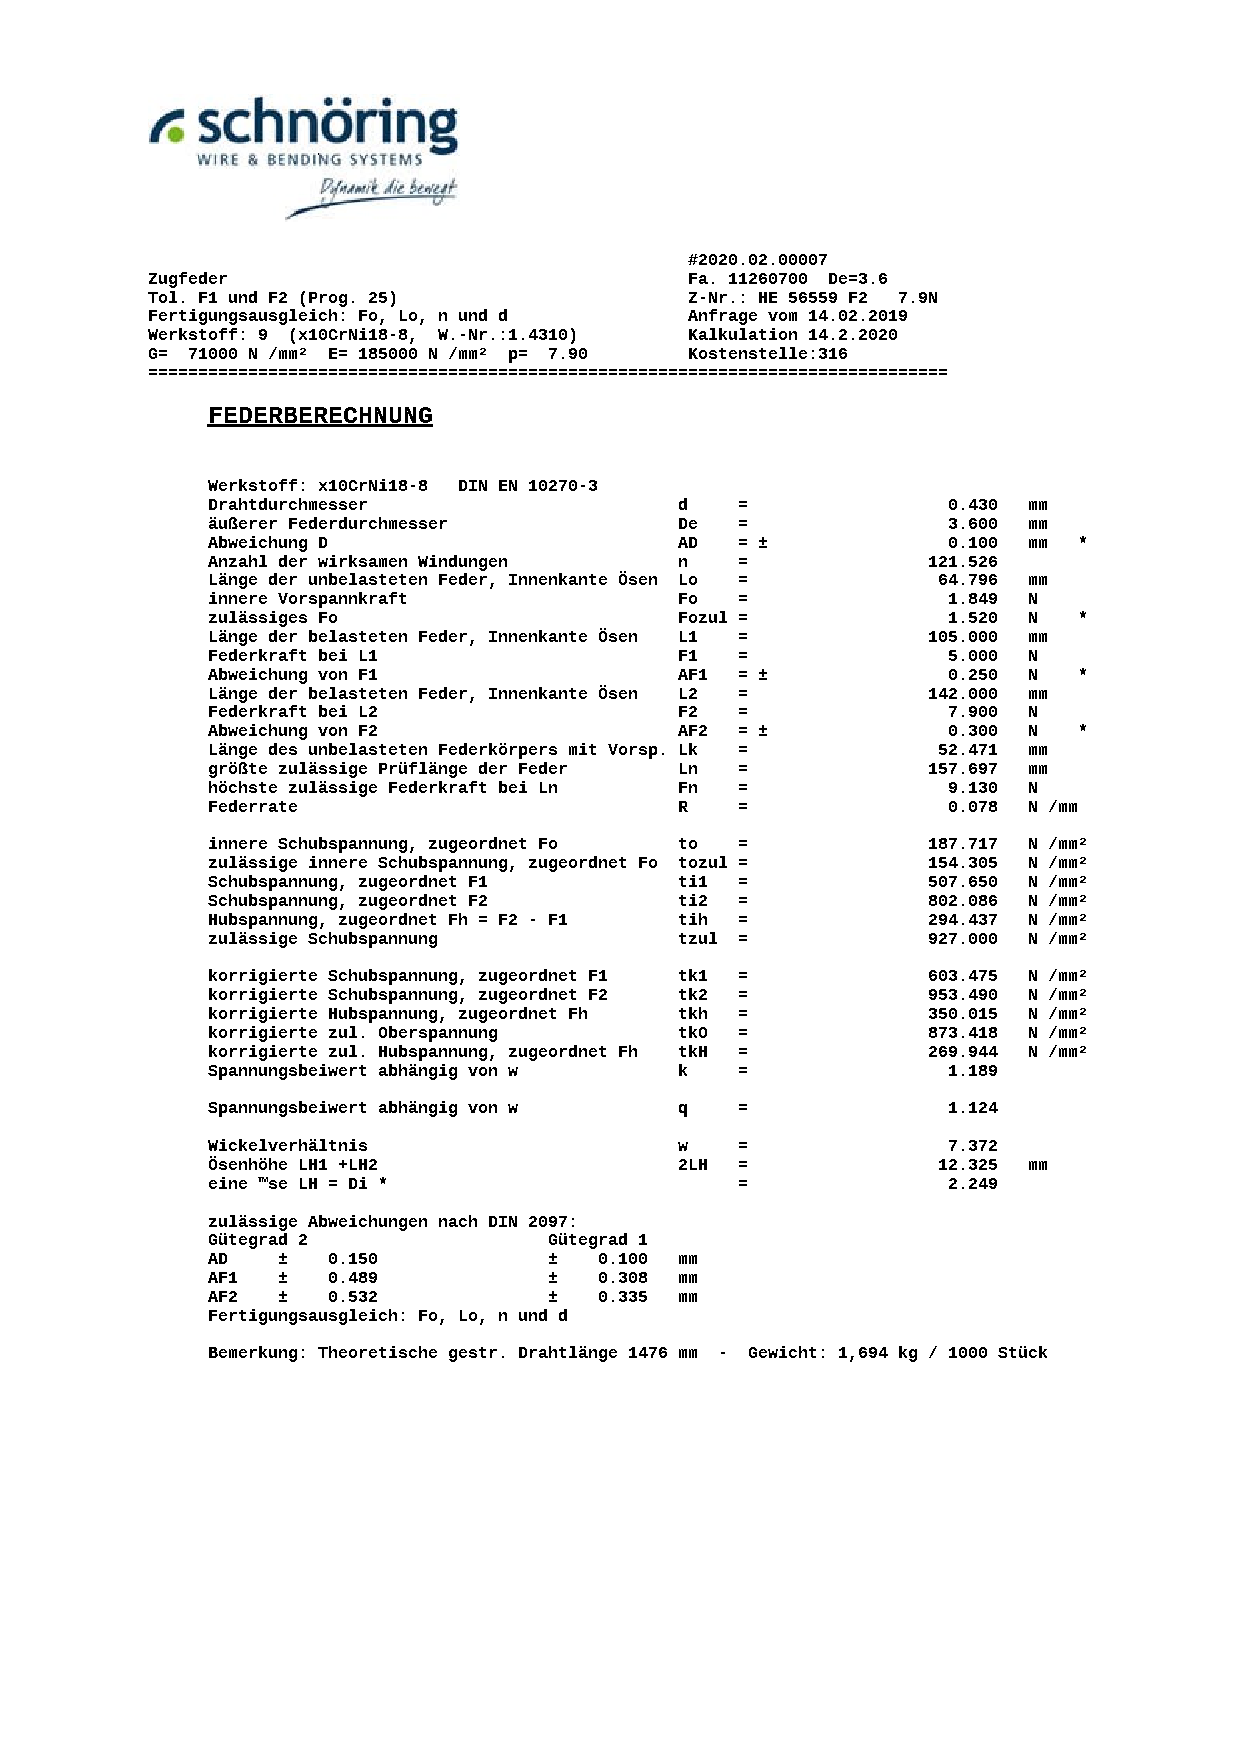
\includegraphics[width=\paperwidth]{bilder/berechnung_De_36.pdf}
%        }
%\end{center}

\newpage
%\nocite{*}
\printbibliography

\end{document}
||||||| merged common ancestors
=======
\documentclass[
  bibliography=totoc,     % Literatur im Inhaltsverzeichnis
  captions=tableheading,  % Tabellenüberschriften
  titlepage=firstiscover, % Titelseite ist Deckblatt
]{scrartcl}

% Paket float verbessern
\usepackage{scrhack}

% Warnung, falls nochmal kompiliert werden muss
\usepackage[aux]{rerunfilecheck}

% unverzichtbare Mathe-Befehle
\usepackage{amsmath}
% viele Mathe-Symbole
\usepackage{amssymb}
% Erweiterungen für amsmath
\usepackage{mathtools}
%einheiten einfügen

% Fonteinstellungen
\usepackage{fontspec}
% Latin Modern Fonts werden automatisch geladen
% Alternativ zum Beispiel:
%\setromanfont{Libertinus Serif}
%\setsansfont{Libertinus Sans}
%\setmonofont{Libertinus Mono}

% Wenn man andere Schriftarten gesetzt hat,
% sollte man das Seiten-Layout neu berechnen lassen
\recalctypearea{}

% deutsche Spracheinstellungen
\usepackage[main=ngerman]{babel}


\usepackage[
  math-style=ISO,    % ┐
  bold-style=ISO,    % │
  sans-style=italic, % │ ISO-Standard folgen
  nabla=upright,     % │
  partial=upright,   % ┘
  warnings-off={           % ┐
    mathtools-colon,       % │ unnötige Warnungen ausschalten
    mathtools-overbracket, % │
  },                       % ┘
]{unicode-math}

% traditionelle Fonts für Mathematik
\setmathfont{Latin Modern Math}
% Alternativ zum Beispiel:
%\setmathfont{Libertinus Math}

\setmathfont{XITS Math}[range={scr, bfscr}]
\setmathfont{XITS Math}[range={cal, bfcal}, StylisticSet=1]

% Zahlen und Einheiten
\usepackage[
  locale=DE,                   % deutsche Einstellungen
  separate-uncertainty=true,   % immer Fehler mit \pm
  per-mode=symbol-or-fraction, % / in inline math, fraction in display math
]{siunitx}

% chemische Formeln
\usepackage[
  version=4,
  math-greek=default, % ┐ mit unicode-math zusammenarbeiten
  text-greek=default, % ┘
]{mhchem}

% richtige Anführungszeichen
\usepackage[autostyle]{csquotes}

% schöne Brüche im Text
\usepackage{xfrac}

% Standardplatzierung für Floats einstellen
\usepackage{float}
\floatplacement{figure}{htbp}
\floatplacement{table}{htbp}

% Floats innerhalb einer Section halten
\usepackage[
  section, % Floats innerhalb der Section halten
  below,   % unterhalb der Section aber auf der selben Seite ist ok
]{placeins}

% Seite drehen für breite Tabellen: landscape Umgebung
\usepackage{pdflscape}

% Captions schöner machen.
\usepackage[
  labelfont=bf,        % Tabelle x: Abbildung y: ist jetzt fett
  font=small,          % Schrift etwas kleiner als Dokument
  width=0.9\textwidth, % maximale Breite einer Caption schmaler
]{caption}
% subfigure, subtable, subref
\usepackage{subcaption}


% Grafiken können eingebunden werden
\usepackage{graphicx}
% größere Variation von Dateinamen möglich
%\usepackage{grffile}

% schöne Tabellen
\usepackage{booktabs}

% Verbesserungen am Schriftbild
\usepackage{microtype}
\setlength{\parindent}{0pt}

% Literaturverzeichnis
\usepackage[
  backend=biber,
]{biblatex}
% Quellendatenbank
\addbibresource{lit.bib}
\addbibresource{programme.bib}

% Hyperlinks im Dokument
\usepackage[
  german,
  unicode,        % Unicode in PDF-Attributen erlauben
  pdfusetitle,    % Titel, Autoren und Datum als PDF-Attribute
  pdfcreator={},  % ┐ PDF-Attribute säubern
  pdfproducer={}, % ┘
]{hyperref}
% erweiterte Bookmarks im PDF
\usepackage{bookmark}

% Trennung von Wörtern mit Strichen
\usepackage[shortcuts]{extdash}

% Import PDFs
\usepackage{pdfpages}


\author{%
  Konstantin Mrozik\\%
  \href{mailto:konstantin.mrozik@udo.edu}{konstantin.mrozik@udo.edu}%
  \and%
  Marcel Kebekus\\%
  \href{mailto:marcel.kebekus@udo.edu}{marcel.kebekus@udo.edu}%
}
\publishers{TU Dortmund – Fakultät Physik}


\title{Zusatzversuch bei Firma Schnöring}
\author{%
  Konstantin Mrozik\\%
  \href{mailto:konstantin.mrozik@udo.edu}{konstantin.mrozik@udo.edu}%
  \and%
  Marcel Kebekus\\%
  \href{mailto:marcel.kebekus@udo.edu}{marcel.kebekus@udo.edu}%
}
\date{%
  Durchführung: 
  \hspace{3em}
  Abgabe: 
}
\publishers{TU Dortmund – Fakultät Physik}
\makeatletter         
\def\@maketitle{
\raggedright
\includegraphics[width=\textwidth]{bilder/lo_TU-Do 2008/logo_rgb_jpg}\\[8ex]
\begin{center}
{\Huge \bfseries \sffamily \@title }\\[4ex] 
{\Large  \@author}\\[4ex] 
\@date\\[8ex]
\publishers\\
\end{center}}
\makeatother


\begin{document}


\maketitle
\thispagestyle{empty}
\tableofcontents
\newpage
\section{Theorie}
\label{sec:Theorie}
Die Fourier Synthese ist eine Methode um eine beliebige Funktion mit einer Summe von Kosinus und Sinus Funktionen zu approximieren.
\begin{align}
    f(t) &= \sum_{k=0}^{\infty} (A_k\cos(\omega_k t)+B_k\sin(\omega_k t)) &   mit \; \omega_k &= \frac{2\pi k}{T}
\end{align}
wobei die Koeffizienten $A_k$ und $B_k$ festgelegt sind durch
\begin{align}
    A_k &= \frac{2}{T} \int_{-T/2}^{+T/2} f(t)\cos(\omega_k t) dt    &  mit \; A_0 &= \frac{1}{T} \int_{-T/2}^{+T/2} f(t) dt \\
    B_k &= \frac{2}{T} \int_{-T/2}^{+T/2} f(t)\sin(\omega_k t) dt    &  mit \; B_0 &= 0
\end{align}
\\
Dabei beschreibt $T$ die Periodendauer, $\omega_k$ die Frequenz und $A_k$ und $B_k$ die zugehörigen Koeffizienten. \\
Im Folgenden soll mit dem Programm Fouriersynthese %Bib setzen
die Funktionen $f(x)=x$ und $f(x)=|sin(x)|$ nachgestellt und die jeweilligen Koeffizienten $B_k$ und $A_k$ ermittelt werden.

\newpage
\section{Durchführung}
\label{sec:Durchfuehrung} %darauf wird verlinkt in Vorbereitungsteil Elastisches Nachwirken!
\subsection{Versuchsaufbau}

\begin{figure}[h]
    \begin{subfigure}[c]{0.5\textwidth}
        \centering
        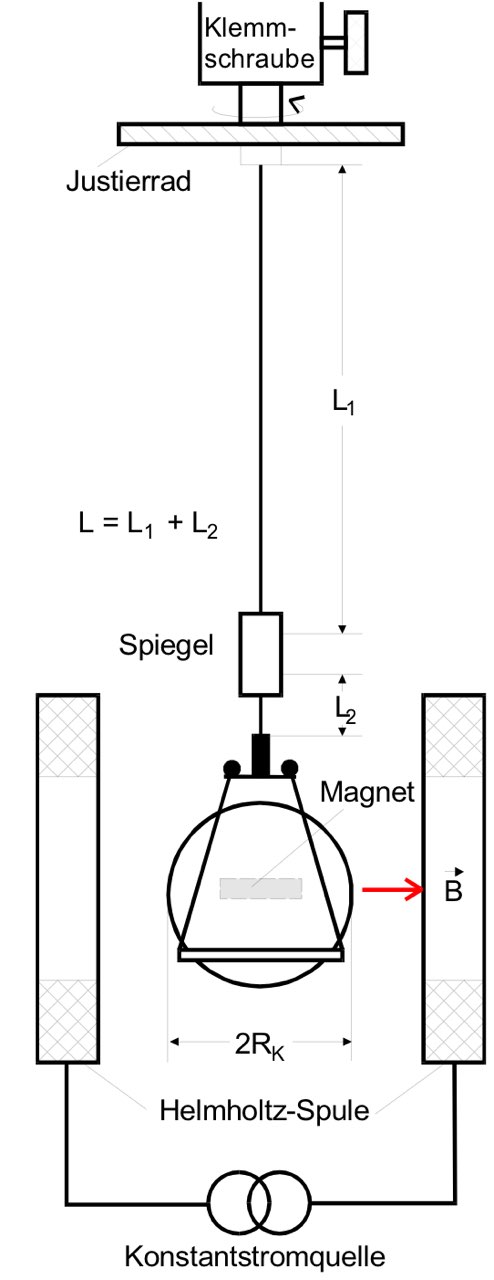
\includegraphics[width=0.3\textwidth, height=0.7\textwidth]{bilder/magnet_apperatur.jpeg}
        \subcaption{Versuchsaufbau Skizze,\cite[9]{Anleitung}}        
        \label{fig:Torsion_apperatur}
    \end{subfigure}
    \begin{subfigure}[c]{0.5\textwidth}
        \centering
        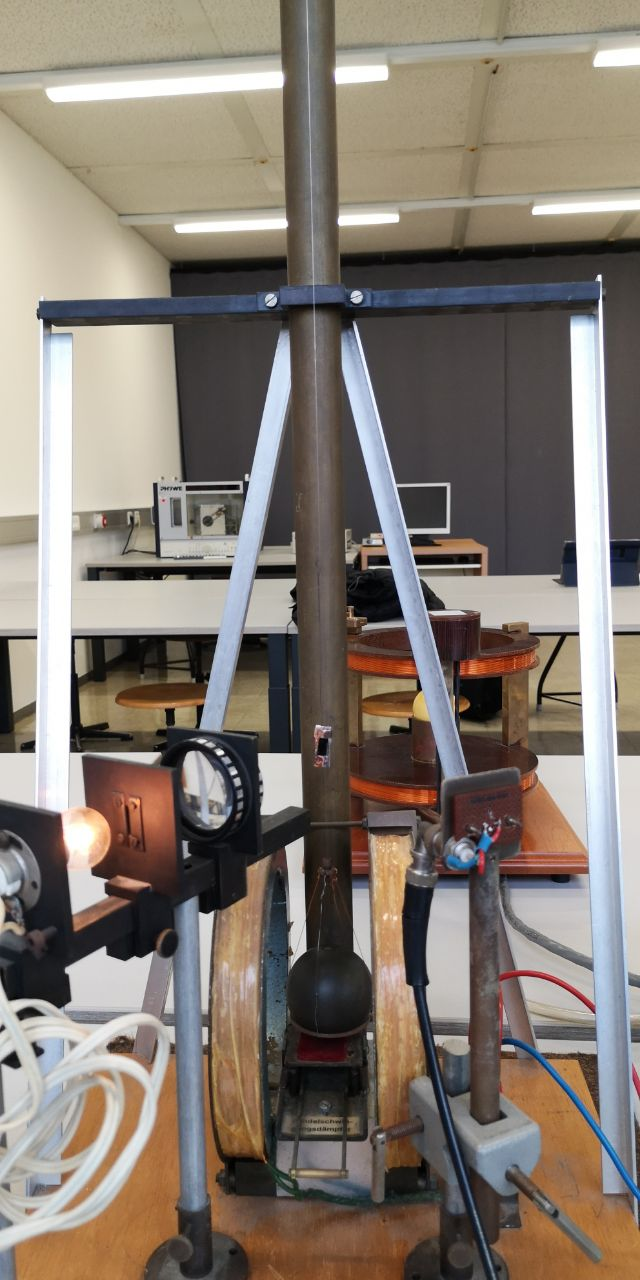
\includegraphics[width=0.3\textwidth, height=0.7\textwidth]{bilder/Foto_Versuchsaufbau.jpeg}
        \subcaption{Foto des Versuchsaufbaus}
        \label{fig:Foto_Versuchsaufbau}
    \end{subfigure}
\end{figure}

Die Kugel soll im Versuch nicht pendeln um Fehler in den Versuchswerten zu vermeiden.
Daher ist unter der Kugel eine Vorrichtung angebracht um nach jeder Messreihe die Pendelbewegung zu dämpfen.\\

Um die Periodendauer zu messen muss mithilfe des Rings an der Aufhängung des Drahtes der Draht verdreht werden,
wobei darauf geachtet werden muss dass der Spiegel bei der Schwingung den Lichtstrahl über die Photodiode lenkt.\\

Das Experiment zur Bestimmung des Elastizitätsmoduls aus der Schallgeschwindigkeit war nicht durchführbar,
daher haben wir hierfür einen vorgegebenen Wert erhalten.\\

\subsection{Die Periodendauer T}
Im ersten Versuch darf an der Helmholtzspule kein Strom anliegen da ausschließlich die Elastizität des Stoffes
 Einfluss auf die Periodendauer haben soll.
Zu Beginn des Versuches wird der Magnet im inneren der Kugel parallel zum Draht eingestellt.
Die Lampe am Versuchsaufbau wird eingeschaltet und das Licht trifft über eine Linse auf den am Draht befestigten Spiegel.
Wenn der Draht nun ausgelenkt wird, läuft der Lichtstrahl über den mitschwingenden Spiegel periodisch über die Photodiode.\\
Die Photodiode ist über eine elektrische Schaltung an die Quarzuhr gekoppelt.
Die elektrische Schaltung lässt über eine bistabile Kippstufe (Flip-Flop) das erste Signal passieren um die Stoppuhr zu starten.
Mithilfe einer weiteren bistabilen Kippstufe wird das 2. Signal unterdrückt.
Das dritte Signal stoppt die Quarzuhr und durch die monostabile Kippstufe und einen weiteren Flip-Flop wird die Uhr mit dem 4. Signal zurück gesetzt.\\
\begin{figure}[h]
    \begin{subfigure}[c]{0.5\textwidth}
        \centering
        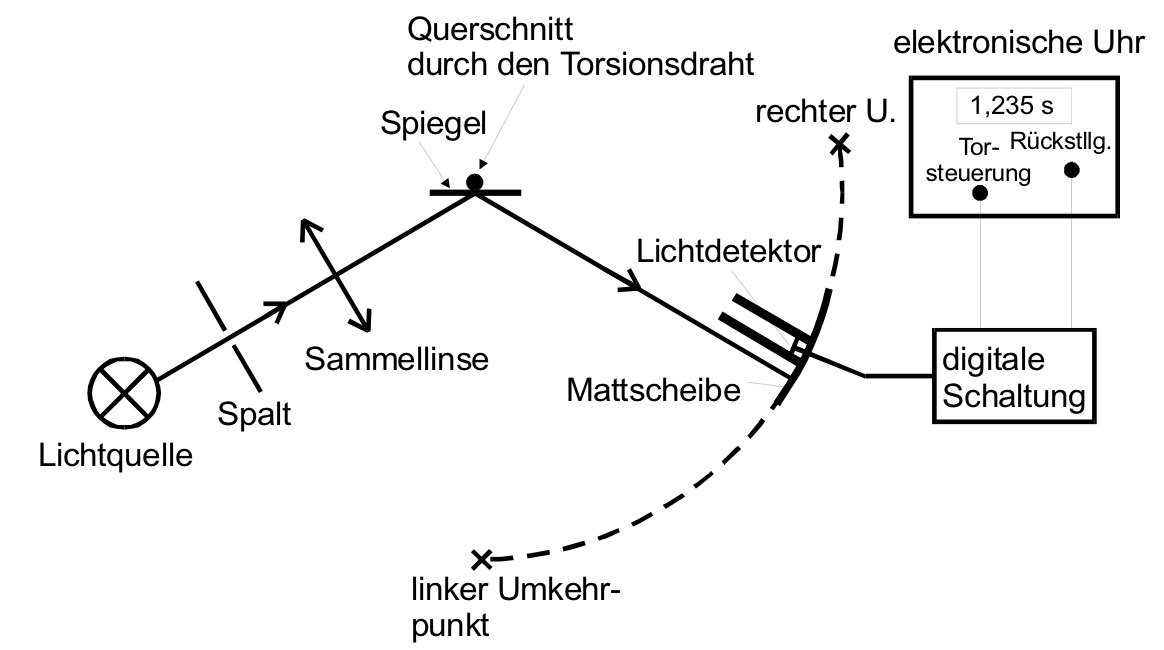
\includegraphics[width=0.7\textwidth, height=0.6\textwidth]{bilder/lichtuhr.jpeg}
        \subcaption{Lichtuhr Skizze,\cite[9]{Anleitung}}        
        \label{fig:lichtuhr}
    \end{subfigure}
    \begin{subfigure}[c]{0.5\textwidth}
        \centering
        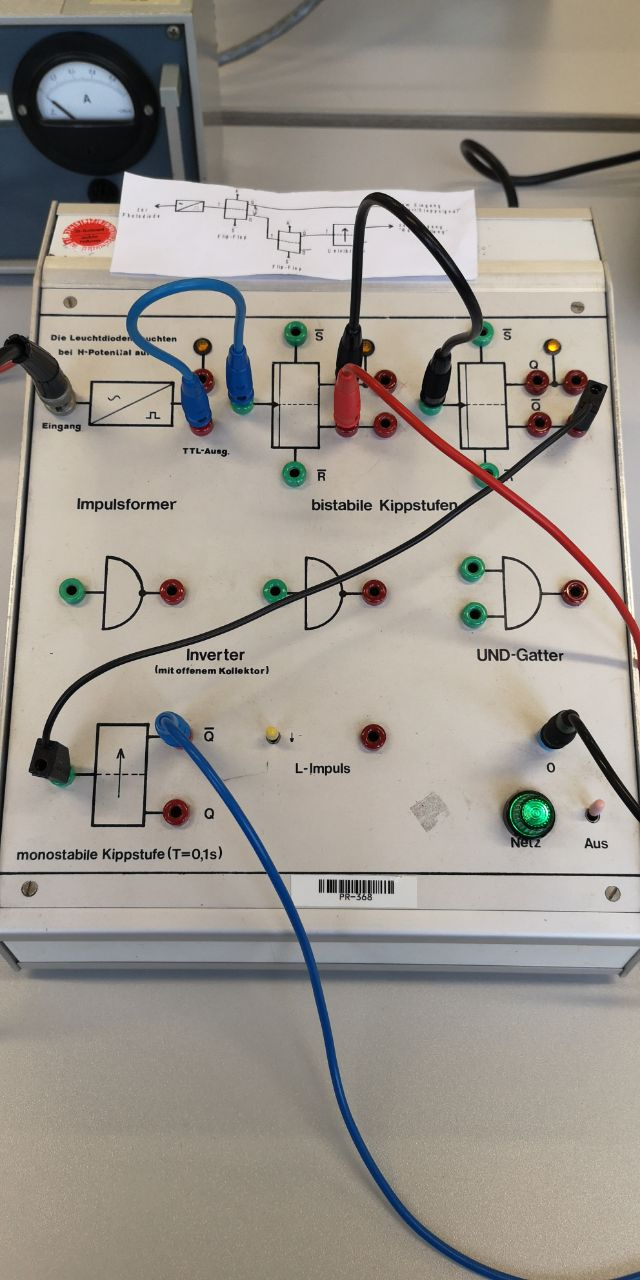
\includegraphics[width=0.45\textwidth, height=0.6\textwidth]{bilder/Schaltung.jpeg}
        \subcaption{Foto der Schaltung}
        \label{fig:Schaltung}
    \end{subfigure}
\end{figure}


\subsection{Die Periodendauer T im B-Feld}
Um die Stärke des Permanentmagneten in der Kugel zu berechnen muss dieser senkrecht zum Draht ausgerichtet werden, da so die Fehler durch das Erdmagnetfeld minimiert werden.
Die Stromstärke an der Helmholtzspule wird nun von 0.1 Ampere bis 1 Ampere in 0.1 Ampere Schritten erhöht und für jede Stromstärke werden 10 Werte gemessen.
%\section{Auswertung}
\label{sec:Auswertung}
\subsection{Bestimmung der Brennweite aus Gegenstandsweite und Bildweite}
Aus dem Mittelwert der gemessenen Werte wird mithilfe von Gleichung \ref{eqn:linsengl} die Brennweite der Linse bestimmt.
\begin{equation}
    f_1 = \frac{g \cdot b}{g+b} = 95,86 \text{mm} \nonumber
\end{equation}
Die Messung wird nun über das auftragen der Messwerte in einem Koordinatensystem bewertet, wenn die Messgenauigkeit hoch ist, sollten sich alle geraden in einem Punkt schneiden dessen x und y koordinate der Brennwite entsprechen.
\begin{figure}[H]
    \centering
    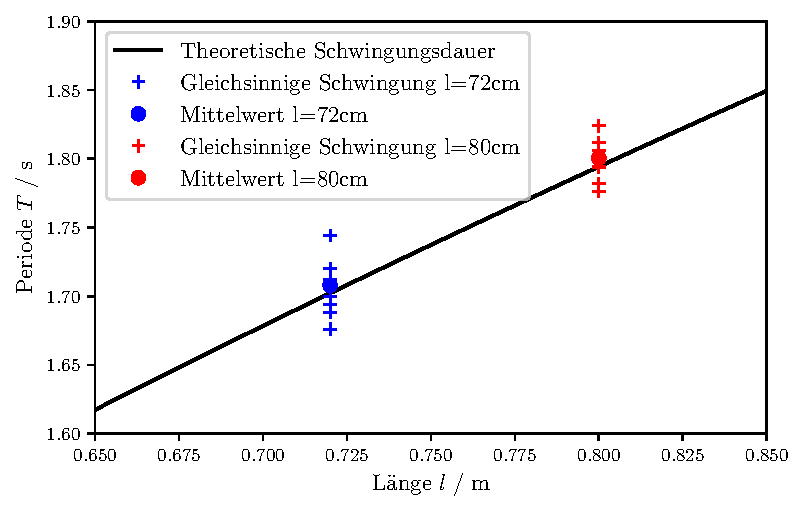
\includegraphics[width=0.6\textwidth]{plots/plot1.pdf}
    \caption{Die Wertepaare werden auf der jeweiligen Achse aufgetragen und durch eine Gerade verbunden}
\end{figure}
Die selbe Methode wird nun auf eine andere Linse mit einer anderen Brennweite angewandt.
Es ergibt sich:
\begin{equation}
    f_2 = 48,07 \text{mm} \nonumber
\end{equation}
Und der entsprachende Graph:
\begin{figure}[H]
    \centering
    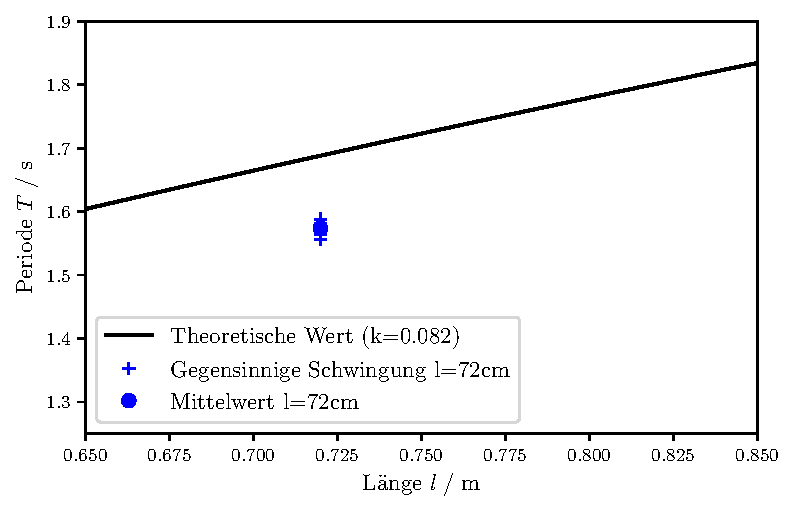
\includegraphics[width=0.6\textwidth]{plots/plot2.pdf}
    \caption{Die Wertepaare werden auf der jeweiligen Achse aufgetragen und durch eine Gerade verbunden}
\end{figure}

\subsection{Methode von Bessel}
Nach der Methode von Bessel lässt sich mit Gleichung \ref{eqn:bessel} die Brennweite der Linse bestimmen.
\begin{table}[H]
    \centering
    \begin{tabular}{c c | c }
        \toprule
        e & d & f\\
        mm & mm & mm\\
        \midrule
        400 & 70 & 96,94\\
        410 & 95 & 97,00\\
        420 & 119& 96,57\\
        430 & 138& 96,43\\
        440 & 155& 96,35\\
        450 & 170& 96,44\\
        460 & 182& 97,00\\
        470 & 193& 97,69\\
        480 & 211& 96,81\\
        490 & 221& 97,58\\
        500 & 233& 97,86 \\
        \bottomrule
    \end{tabular}
    \caption{Die Parameter e und b und die jeweilige berechnete Brennweite}
    \label{tab:tab1}
\end{table}
Als Mittelwert der berechneten Brennweiten ergibt sich
\begin{equation}
    f_{\text{bessel}} = 96,97 \text{mm} \nonumber
\end{equation}
\subsection{Methode von Abbe}
Bei der Methode von Abbe werden die g' und b' aus Gleichung \ref{eqn:abbe1} und \ref{eqn:abbe2} gegen den ensprechenden Term mit V aufgetragen und der lineare Zusammenhang wird untersucht.
\begin{figure}[H]
    \centering
    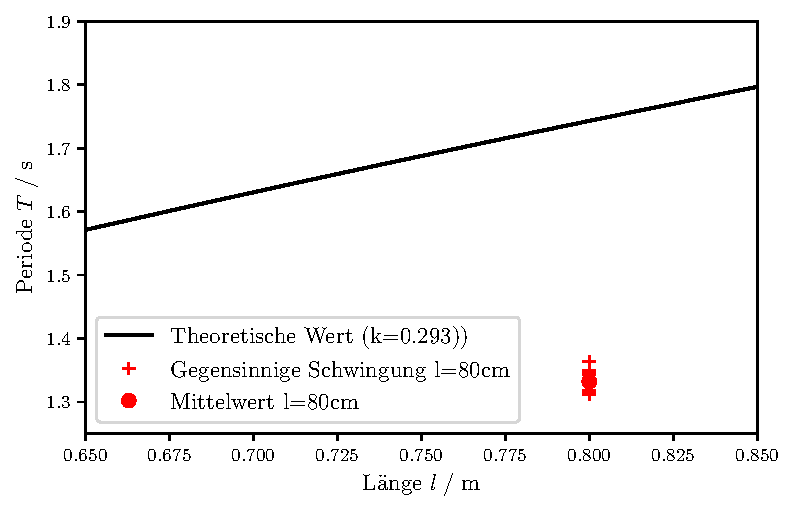
\includegraphics[width=0.6\textwidth]{plots/plot3.pdf}
    \caption{Abbe}
\end{figure}
\begin{figure}[H]
    \centering
    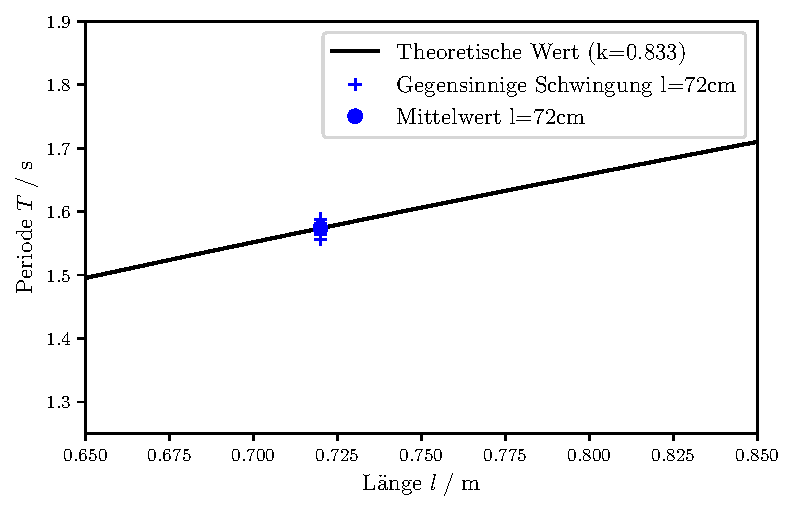
\includegraphics[width=0.6\textwidth]{plots/plot4.pdf}
    \caption{Abbe}
\end{figure}
Bei den hier gemessenen Werten lässt sich nur schwer ein linearer Zusammenhang erkennen.
%\section{Diskussion}
\label{sec:Diskussion}

In der Auswertung kam es bereits zu einigen unrealistischen und offensichtlichen
falschen Werten die alle aus Berechnungen stammten.
Im Folgenden soll die Ursache für die dramastischen Abweichungen analysiert werden.


Dafür soll zu Beginn die Messung an sich überprüft werden.
Dazu wird die jeweilige theoretische Schwingungsdauer mit den gemessenen Schwingungsdauern verglichen.
\begin{figure}
    \centering
    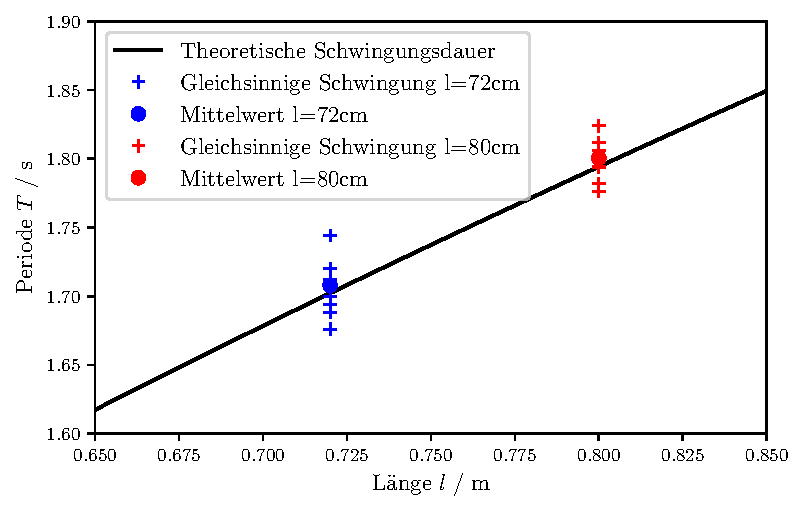
\includegraphics[width=0.5\textwidth]{plots/plot1.pdf}
    \caption{Gleichsinnige Schwingungen}
\end{figure}
Die Theoretische Kurve folgt aus Glichung (6!). Es wird deutlich, dass die gemessenen
Schwingungsdauern $T_+$ mit den zu erwartenen Schwingungsdauern übereinstimmt.\\

Für die Gegensinnige Schwingung ergibt sich der zu erwartende Theoretische Werte aus Geichung (8!).

\begin{figure}
    \begin{subfigure}[c]{0.5\textwidth}
        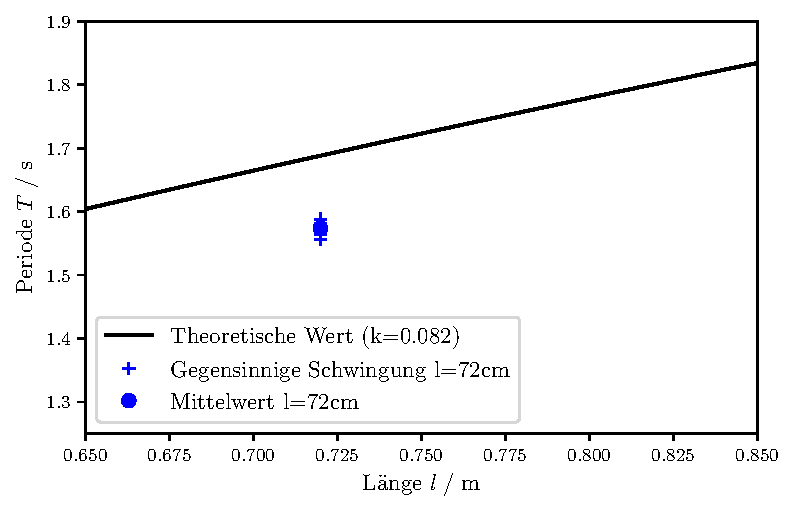
\includegraphics[width=\textwidth]{plots/plot2.pdf}
        \subcaption{Pedel 72cm}
    \end{subfigure}
    \begin{subfigure}[c]{0.5\textwidth}
        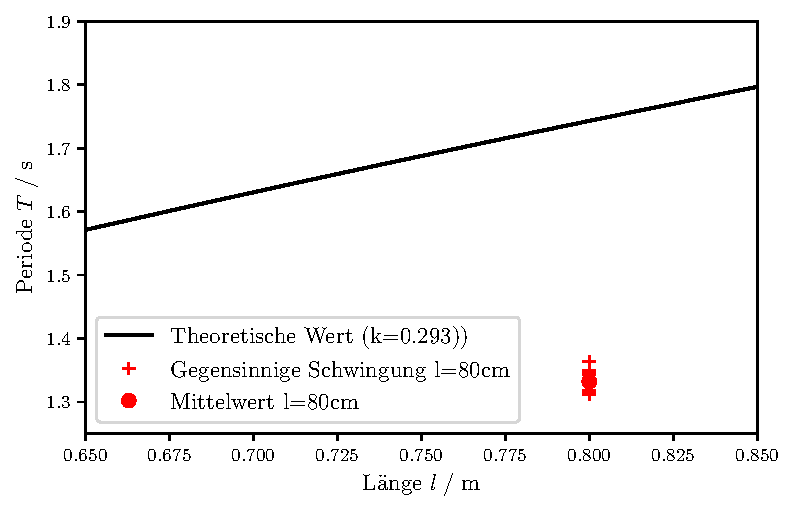
\includegraphics[width=\textwidth]{plots/plot3.pdf}
        \subcaption{Pendel 80cm}
        \label{subfig:pedel80}
    \end{subfigure}
    \caption{Gegensinnige Schwingungsdauer}
\end{figure}

Hier bei wird besonders gut deutlich, dass bei \ref{subfig:pendel80}, große Abweichungen
vorliegen. Dies lässt sich nur auf einen Messfehler zurückführen.
Weiterführend sei zu beachten, dass die Kopplungskonstante die für die theoretische Kurve
verwendet wird, ebenfalls aus diesen falschen Werten stammt.

Dies erklärt weiterführend, warum die Kopplungskonstant aus \ref{eqn:kopplung80} nicht die selben
sind.
Behauptung: Der Messfehler der Gegensinnigen Schwingung von der Pendellänge $l=80cm$ und $l=72cm$ ist 
ist ein Ursprung der Fehler.

Stellt man Gleichung (\ref{eqn:T_m}) um, um die Größenordung der Kopplungskonstante $K$ zu erörtern, so gilt:
\begin{equation}
    K=\frac{2\pi^2l}{T_{-}^2}-\frac{g}{2}
\end{equation}
Somit ergibt sich:
\begin{align*}
    \textrm{K für 72cm} = 0,833\\
    \textrm{K für 80cm} = 3,995 
\end{align*}
Für diese neuen Kopplungskonstanten sei gesagt, dass sie nur als Größenordnung diehnen.
Denn durch die passenden gleichsinnigen Schwingungsdauern $T_+$und den fehlerhaften gegensinnigen Schwingungsdauern $T_-$
folgt nach Gleichung (\ref{eqn:Kopplungkonstante}) eine fehlerhaft Kopplungkonstante $K$.
 
Trägt man für diese neuen Kopplungskonstanten die gegensinnigen Schwingungen auf, dies Bestätig die Annahme
das der Fehler in den gemessenen gegenphasigen Schwingungsdauern.  
\begin{figure}
    \begin{subfigure}[c]{0.5\textwidth}
        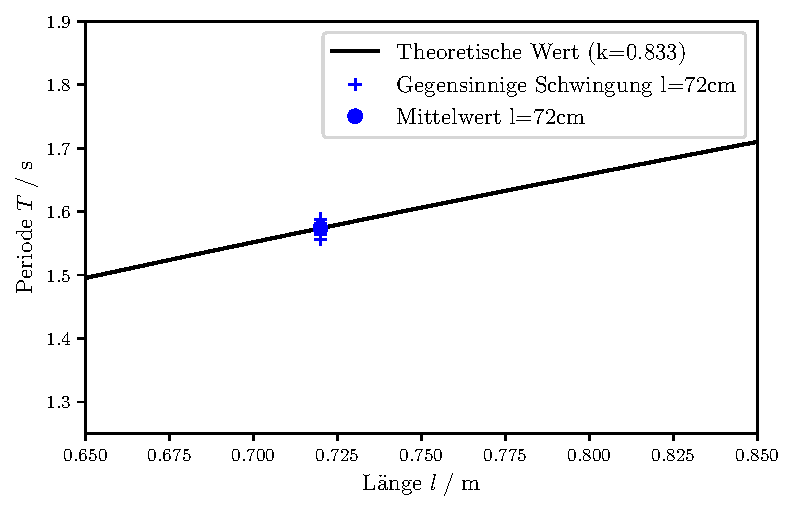
\includegraphics[width=\textwidth]{plots/plot4.pdf}
        \subcaption{Pedel 72cm}
    \end{subfigure}
    \begin{subfigure}[c]{0.5\textwidth}
        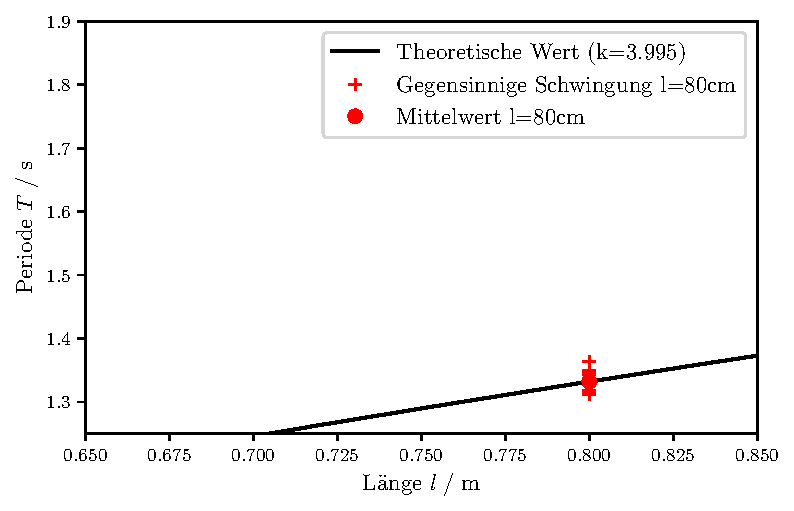
\includegraphics[width=\textwidth]{plots/plot5.pdf}
        \subcaption{Pendel 80cm}
        \label{subfig:gegenNEU80}
    \end{subfigure}
    \caption{Gegensinnige Schwingungsdauer mit Kopplungskonstante}
\end{figure}

Fazit: Der Fehler findet sich beim Messen der gegensinnigen Schwingungen und
zieht sich dann durch die Rechnungen für die Kopplungskonstante $K$ und die Frequenzen $\omega$
so wie für die Schwebungsdauer.\\
Somit stimmen gemessene und berechnete Werte nicht überein.



%\newpage
\nocite{*}
\printbibliography

\end{document}
>>>>>>> 4725ae2bea169a0e96b27f3c21c1fb3c50c57da5
